\renewcommand{\theequation}{\theenumi}
\begin{enumerate}[label=\arabic*.,ref=\thesubsubsection.\theenumi]
\numberwithin{equation}{enumi}
\item For a general polynomial equation of degree 2 , \\
$p(x,y) \implies Ax^2+Bxy+Cy^2+Dx+Ey+F=0$ \\
The vector form is  
\begin{align}
\vec{x}^T\myvec{A&B/2\\B/2&C}\vec{x}+\myvec{D&E}\vec{x}+F=0 \label{eq:poly}
\end{align} 

\begin{enumerate}

\item $x^2-3x-10=0$  \\
The vector form from the equation is \ref{eq:poly} is 
\begin{align}
\vec{x}^T\myvec{1&0\\0&0}\vec{x}+\myvec{-3&0}\vec{x}-10=0
\end{align}

The values of $\vec{x}$ are found in the following python code
\begin{lstlisting}
codes/conics/exercise/conics_1.py
\end{lstlisting}

$\vec{x}=\myvec{5\\0}, \myvec{-2\\0}$ \\
which can be verified from the Fig.\ref{fig:parabola_1}.
The following python code generates the fig.\ref{fig:parabola_1}
\begin{lstlisting}
codes/conics/exercise/conics_1.py
\end{lstlisting}
\begin{figure}[!ht]
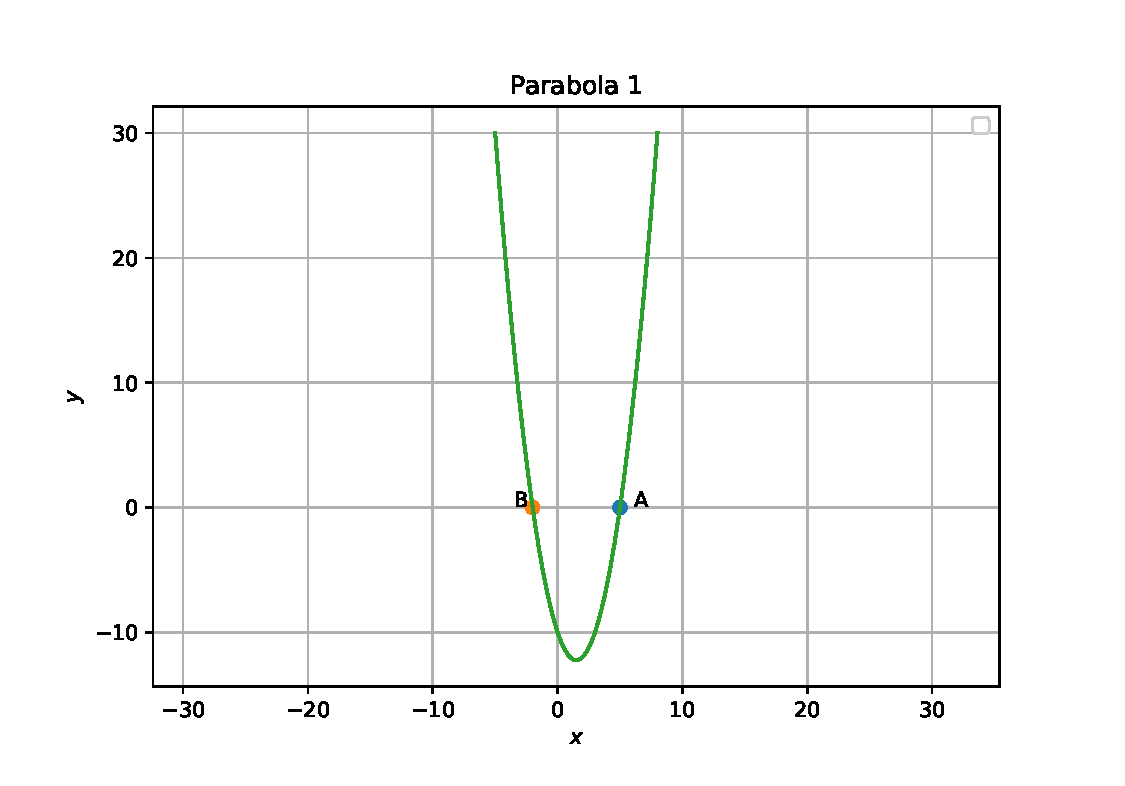
\includegraphics[width=\columnwidth]{./codes/conics/exercise/conics_1.eps}
\caption{Parabola 1}
\label{fig:parabola_1}
\end{figure} 

\item $2x^2+x-6=0$ \\
The vector form from the equation is \ref{eq:poly} is
\begin{align}
\vec{x}^T\myvec{2&0\\0&0}\vec{x}+\myvec{1&0}\vec{x}-6
=0
\end{align}
The values of $\vec{x}$ are found in the following python code
\begin{lstlisting}
codes/conics/exercise/conics_2.py
\end{lstlisting}

$\vec{x}=\myvec{1.5\\0}, \myvec{-2\\0}$ \\
which can be verified from the Fig.\ref{fig:parabola_2}.
The following python code generates the fig.\ref{fig:parabola_2}
\begin{lstlisting}
codes/conics/exercise/conics_2.py
\end{lstlisting}
\begin{figure}[!ht]
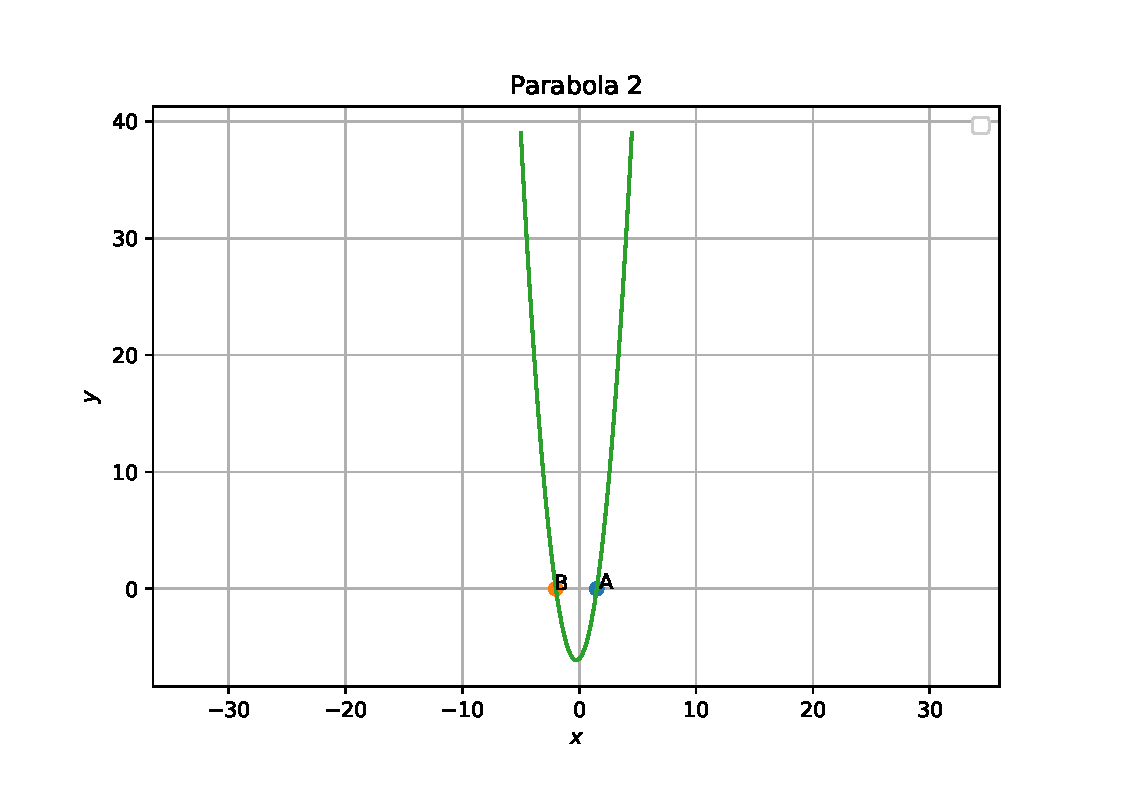
\includegraphics[width=\columnwidth]{./codes/conics/exercise/conics_2.eps}
\caption{Parabola 2}
\label{fig:parabola_2}
\end{figure} 

\item $\sqrt{2}x^2+7x+5\sqrt{2}=0$ \\
The vector form from the equation is \ref{eq:poly} is
\begin{align}
\vec{x}^T\myvec{\sqrt{2}&0\\0&0}\vec{x}+\myvec{7&0}\vec{x}+5\sqrt{2}=0
\end{align}
 
The values of $\vec{x}$ are found in the following python code
\begin{lstlisting}
codes/conics/exercise/conics_3.py
\end{lstlisting}

$\vec{x}=\myvec{-1.414\\0}, \myvec{-3.535\\0}$
which can be verified from the Fig.\ref{fig:parabola_3}.
The following python code generates the fig.\ref{fig:parabola_3}
\begin{lstlisting}
codes/conics/exercise/conics_3.py
\end{lstlisting}
\begin{figure}[!ht]
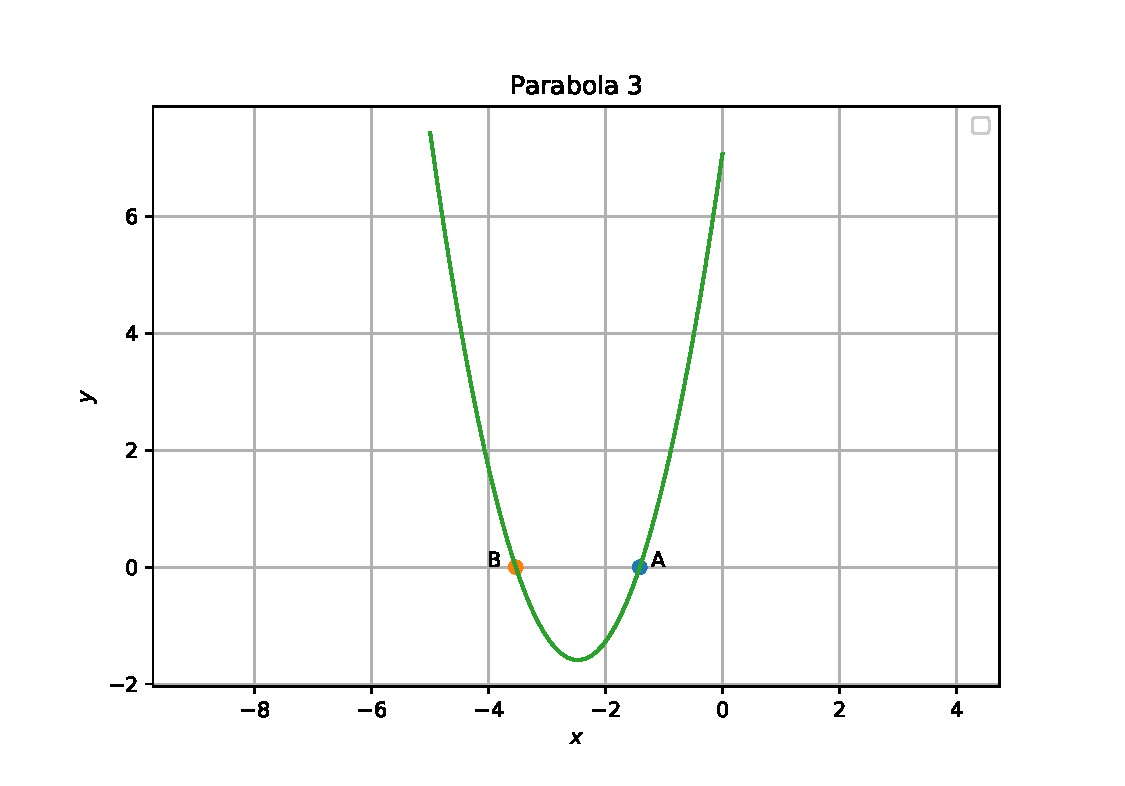
\includegraphics[width=\columnwidth]{./codes/conics/exercise/conics_3.eps}
\caption{Parabola 3}
\label{fig:parabola_3}
\end{figure} 

\item $2x^2-x+\frac{1}{8}=0$ \\
The vector form from the equation is \ref{eq:poly} is
\begin{align}
\vec{x}^T\myvec{2&0\\0&0}\vec{x}+\myvec{-1&0}\vec{x}+\frac{1}{8}=0
\end{align}

The values of $\vec{x}$ are found in the following python code
\begin{lstlisting}
codes/conics/exercise/conics_4.py
\end{lstlisting}

$\vec{x}=\myvec{0.25\\0}, \myvec{0.25\\0}$ \\
which can be verified from the Fig.\ref{fig:parabola_4}.
The following python code generates the fig.\ref{fig:parabola_4}
\begin{lstlisting}
codes/conics/exercise/conics_4.py
\end{lstlisting}
\begin{figure}[!ht]
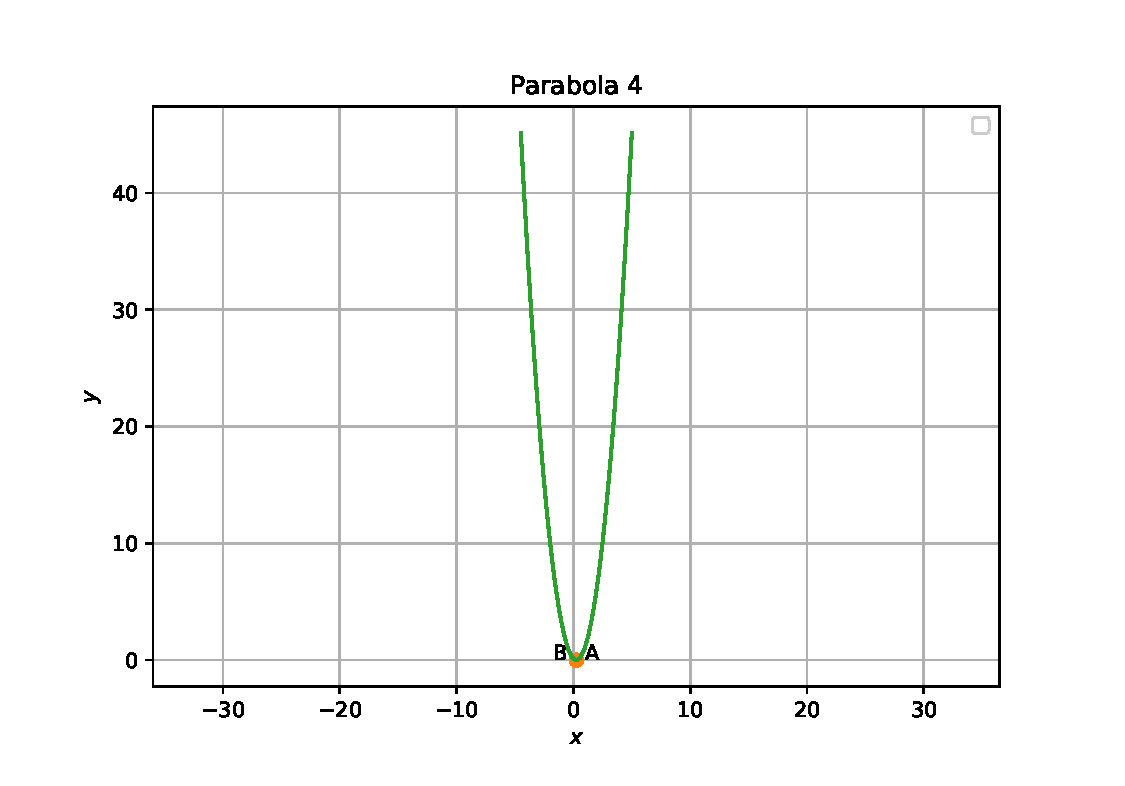
\includegraphics[width=\columnwidth]{./codes/conics/exercise/conics_4.eps}
\caption{Parabola 4}
\label{fig:parabola_4}
\end{figure} 


\item $100x^2-20x+1=0$ \\
The vector form from the equation is \ref{eq:poly} is
\begin{align}
\vec{x}^T\myvec{100&0\\0&0}\vec{x}+\myvec{-20&0}\vec{x}+1=0
\end{align}

The values of $\vec{x}$ are found in the following python code
\begin{lstlisting}
codes/conics/exercise/conics_5.py
\end{lstlisting}

$\vec{x}= \myvec{0.1\\0}, \myvec{0.1\\0}$
which can be verified from the Fig.\ref{fig:parabola_5}.
The following python code generates the fig.\ref{fig:parabola_5}
\begin{lstlisting}
codes/conics/exercise/conics_5.py
\end{lstlisting}
\begin{figure}[!ht]
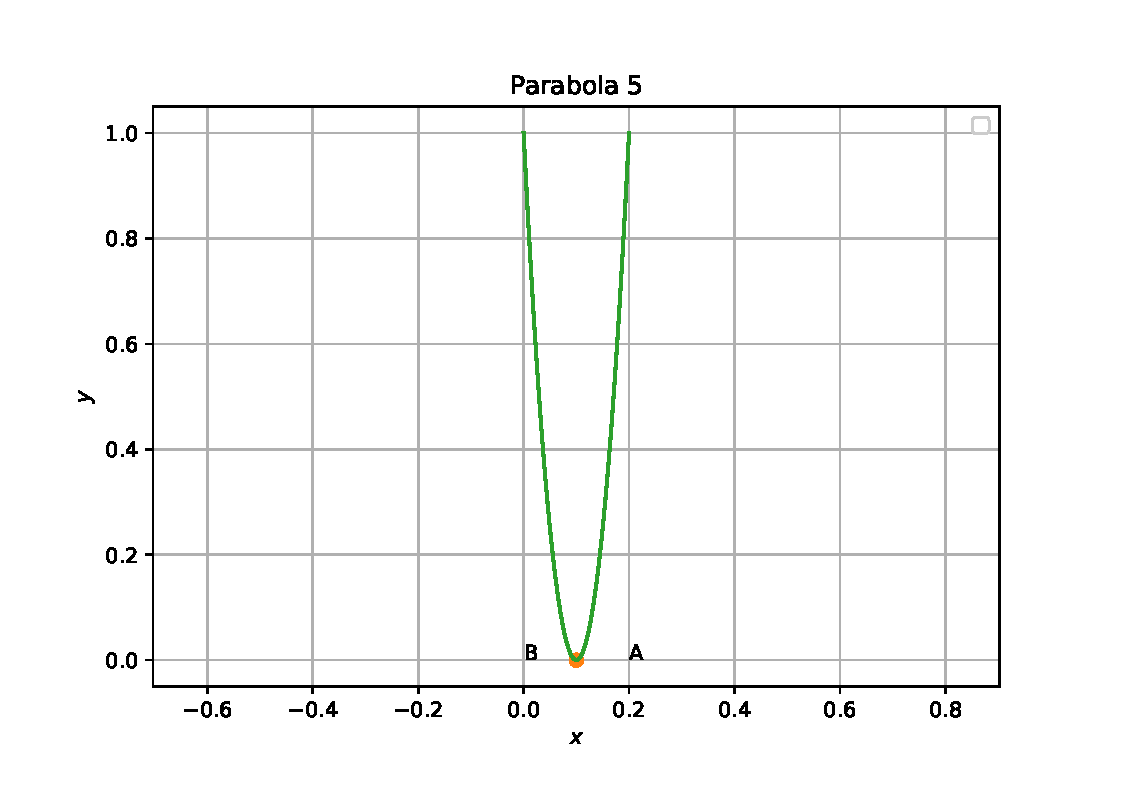
\includegraphics[width=\columnwidth]{./codes/conics/exercise/conics_5.eps}
\caption{Parabola 5}
\label{fig:parabola_5}
\end{figure} 

\end{enumerate}

\end{enumerate}